
\subsubsection{Delegat}
\label{sec:patro_delegat}

El delegat és un patró de disseny simple i molt potent. L'objecte que s'ha delegat manté una referència cap a l'altre objecte (el delegat) i li pot enviar missatges.
El missatge informen d'algun fet succeït, donant l'oportunitat al delegat de reaccionar davant d'aquests fets. El delegat pot respondre al missatge actualitzant el seu estat o l'estat d'altres objectes de l'aplicació. El principal valor de la delegació és que permet personalitzar fàcilment el comportament de diversos objectes amb un objecte central.

\begin{figure}[ht]
    \centering
    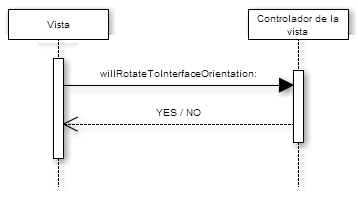
\includegraphics[scale=1]{Memoria/Arquitectura/iOS/patro_delegat.png}
    \caption{Comunicació vista-controlador mitjançant delegats.}
    \label{fig:patro_delegat}
\end{figure}


Un exemple d'objecte delegat és un controlador de vista d'una aplicació d'\textit{iOS}. Totes les vistes tenen declarat un protocol, on uns dels mètodes delegats és ``willRotateToInterfaceOrientation:''. Quan el dispositiu va a rotar, la vista afectada per la rotació li envia al seu delegat ``willRotateToInterfaceOrientation'' per a que el controlador de vista respongui si ha de girar o no. Es pot veure un esquema en la figura \ref{fig:patro_delegat}.